\begin{align}\label{eq:solution/line_plane/822}
   \vec{n}^T\vec{x} = c
\end{align}
where $\vec{n}$=normal vector to the plane
The distance from the origin is given by:-
\begin{align}
    \frac{\abs{c}}{\norm{\vec{n}}} = 7\label{eq:solution/line_plane/823}\\
    \norm{\vec{n}}=\sqrt{3^2+5^2+6^2}=\sqrt{70}\label{eq:solution/line_plane/824}
\end{align}
Substituting equation \eqref{eq:solution/line_plane/824} in \eqref{eq:solution/line_plane/823} we get,
\begin{align}
    \frac{\abs{c}}{\sqrt{70}}=7\label{eq:solution/line_plane/825}\\
    c=\pm{7\sqrt{70}}\label{eq:solution/line_plane/826}
\end{align}
Substituting equation \eqref{eq:solution/line_plane/821},\eqref{eq:solution/line_plane/826} in \eqref{eq:solution/line_plane/822} we get two equation of planes,
\begin{align}
    \boxed{\myvec{3 & 5 & 6}\vec{x}=7\sqrt{70}}\label{eq:solution/line_plane/827}\\
     \boxed{\myvec{3 & 5 & 6}\vec{x}=-7\sqrt{70}}\label{eq:solution/line_plane/828}
\end{align}
Equation \eqref{eq:solution/line_plane/827} and \eqref{eq:solution/line_plane/828} gives us the equation of two planes which are at a distance of 7 units from origin and normal to $\myvec{3\\5\\6}$
%\begin{figure}[h!]
%	\centering
%	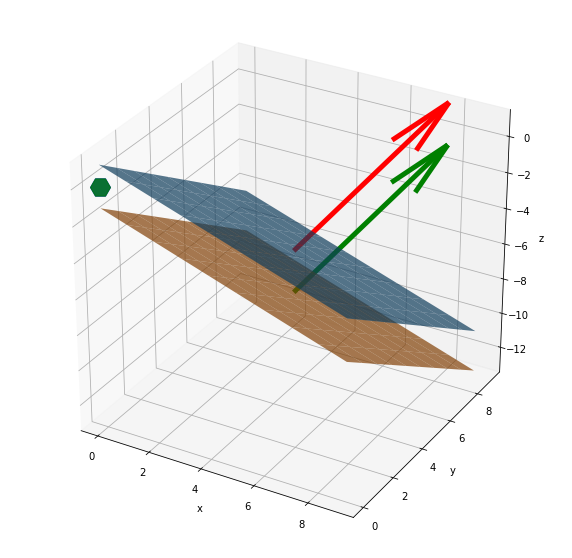
\includegraphics[width=\columnwidth]{plane.png}
%	\caption{Planes with Normal vectors}
%	\label{eq:solution/line_plane/82myfig}
%\end{figure}
%\end{document}
